\chapter{Integración con el frontend y pruebas de extremo a extremo}\label{cap:frontend}

El frontend (Next.js~16, React~19 y Zustand) se diseñó desde el principio con la forma del contrato: montos en centavos, los mismos estados del plan y los mismos códigos de error. En esta etapa se reemplazaron sus datos de prueba por llamadas a la API desplegada en AWS y se publicó en Azure App Service. Así la solución quedó repartida en dos nubes: la API y su Gateway en AWS, y la aplicación web en Azure.

\section{Arquitectura de la integración}

\begin{table}[H]
\centering
\caption{Piezas del frontend que consumen la API}\label{tab:front-piezas}
\begin{tabularx}{\linewidth}{@{}>{\ttfamily\raggedright}p{3.6cm} X@{}}
\toprule
\textbf{\normalfont Pieza} & \textbf{Responsabilidad} \\
\midrule
lib/api.ts & Cliente HTTP. Agrega el access token, genera la \texttt{Idempotency-Key} en las operaciones que crean recursos o mueven dinero, renueva el token una vez ante un 401 y convierte las respuestas \texttt{application/problem+json} en errores con el \texttt{codigo} del contrato. \\
lib/auth-store.ts & Sesión: \texttt{POST /v1/auth/token} con contraseña o refresh token y \texttt{GET /v1/clientes/me}. Si varias peticiones reciben 401 a la vez, comparten una sola renovación. \\
lib/store.ts & Estado de la aplicación conectado a la API: planes con su resumen, cuentas, tarifas, movimientos por cursor y las acciones sobre el plan. \\
next.config.ts & Proxy del mismo origen: \texttt{/api/*} se reenvía al API Gateway. \\
\bottomrule
\end{tabularx}
\end{table}

\paragraph{Proxy del mismo origen.} Azure sirve el frontend solo por HTTPS, y el navegador bloquea las llamadas de una página HTTPS a un servidor HTTP (contenido mixto). Por eso el navegador no llama directamente al Gateway: llama a \texttt{/api/...} en el mismo dominio, y el servidor de Next.js reenvía la petición a AWS. Con este diseño tampoco hace falta CORS. Al exponer el Gateway directamente al navegador durante el desarrollo apareció un problema: el plugin \texttt{jwt} de Kong rechazaba la verificación previa de CORS (\texttt{OPTIONS}), que no lleva token. Se corrigió con \texttt{run\_\allowbreak{}on\_\allowbreak{}preflight: false}, para que esas peticiones las atienda el plugin \texttt{cors}.

\begin{table}[H]
\centering
\caption{Operaciones del contrato que usa cada pantalla}\label{tab:front-pantallas}
\begin{tabularx}{\linewidth}{@{}>{\raggedright}p{3.2cm} X@{}}
\toprule
\textbf{Pantalla} & \textbf{Operaciones} \\
\midrule
Ingreso & \texttt{POST /v1/auth/token}, \texttt{GET /v1/clientes/me} \\
Dashboard & \texttt{GET /v1/planes-ahorro} (con \texttt{resumen}), \texttt{GET /v1/cuentas-debito} \\
Nuevo plan & \texttt{GET /v1/simulaciones}, \texttt{GET /v1/cuentas-debito}, \texttt{POST /v1/planes-ahorro} \\
Detalle del plan & \texttt{GET /v1/planes-ahorro/\{id\}}, \texttt{GET /\{id\}/movimientos} (cursor), \texttt{GET /v1/tarifas}, \texttt{POST /\{id\}/bloqueo}, \texttt{/desbloqueo} y \texttt{/cancelacion} \\
Aportar y retirar & \texttt{POST /\{id\}/aportes} y \texttt{/retiros} (202), \texttt{GET} de la URL indicada en \texttt{Location} \\
\bottomrule
\end{tabularx}
\end{table}

\section{Operaciones asíncronas en la interfaz}

Un aporte o un retiro responde \texttt{202 Accepted} con la cabecera \texttt{Location} del recurso creado. La interfaz muestra ``Esperando la confirmación del banco'' y consulta esa URL cada 800~ms, durante 15~s como máximo, hasta que el estado deja de ser \texttt{PENDIENTE}:

\begin{itemize}
  \item \texttt{EJECUTADO}: se recargan el plan, el historial, el resumen y los saldos de las cuentas.
  \item \texttt{FALLIDO}: se muestra el motivo (\texttt{FONDOS\_\allowbreak{}INSUFICIENTES}, \texttt{CUENTA\_\allowbreak{}BLOQUEADA} o \texttt{CORE\_\allowbreak{}NO\_\allowbreak{}DISPONIBLE}) en lenguaje del usuario.
  \item Sin respuesta dentro de los 15~s: se informa que el banco sigue procesando la operación y que se reflejará en unos segundos.
\end{itemize}

La simulación del plan nuevo se pide al servidor (\texttt{GET /v1/simulaciones}) cuando el usuario deja de escribir durante 400~ms. Así la cuota y las tasas salen de la misma estrategia de cálculo que usa el backend, y no se consume el límite de peticiones en cada tecla.

\section{Despliegue en Azure}

\begin{table}[H]
\centering
\caption{Recursos del frontend en Azure}\label{tab:azure}
\begin{tabularx}{\linewidth}{@{}>{\raggedright}p{3.6cm} X@{}}
\toprule
\textbf{Recurso} & \textbf{Configuración} \\
\midrule
Suscripción & Azure for Students. Su política solo permite cinco regiones; se eligió \texttt{canadacentral}, la más cercana a la API en \texttt{us-east-2}. \\
Plan de App Service & \texttt{billetera-ahorro-plan}, Linux, nivel F1 (gratuito). \\
Aplicación web & \texttt{billetera-ahorro-front}: Node~24 LTS, servidor \texttt{standalone} de Next.js (\texttt{node server.js}), solo HTTPS, TLS mínimo 1.3 y FTP deshabilitado. \\
Identidad para CI/CD & Identidad administrada \texttt{billetera-ahorro-github} con credencial federada (OIDC) para la rama \texttt{main} del repositorio (el \emph{subject} incluye los identificadores numéricos del dueño y del repositorio, formato que GitHub envía para este repositorio) y el rol \emph{Website Contributor} limitado al grupo de recursos. No hay contraseñas guardadas en GitHub. \\
\bottomrule
\end{tabularx}
\end{table}

Dos workflows de GitHub Actions completan el despliegue:

\begin{itemize}
  \item \textbf{Frontend CI/CD} (\texttt{frontend-ci-cd.yml}): lint, verificación de tipos y compilación; empaqueta el servidor \texttt{standalone}, lo despliega en App Service y verifica que la aplicación responda. Si la aplicación está apagada, omite el despliegue en lugar de fallar.
  \item \textbf{Azure - encender o apagar} (\texttt{azure-frontend.yml}): enciende, apaga o consulta la aplicación y, opcionalmente, la instancia EC2 del backend. Así la demostración se levanta con un solo clic y fuera de ella no se consumen recursos.
\end{itemize}

La primera ejecución del pipeline del frontend reveló dos problemas que no aparecían en el entorno local:
\begin{itemize}
  \item La verificación de tipos fallaba porque los tipos globales de Next.js (\texttt{.next/types}) no existen en un checkout limpio. Se agregó \texttt{next typegen} antes de \texttt{tsc}.
  \item El inicio de sesión en Azure fallaba (\texttt{AADSTS700213}), porque GitHub envía para este repositorio un \emph{subject} OIDC con los identificadores numéricos del dueño y del repositorio. Se ajustó la credencial federada.
\end{itemize}
Con ambas correcciones, el pipeline compiló, desplegó en App Service y verificó el sitio. Después, el workflow de encendido y apagado detuvo la aplicación web y la instancia EC2 en una sola ejecución (Anexo~\ref{anx:evidencias}).

Las verificaciones del Anexo~\ref{anx:evidencias} confirman lo siguiente:
\begin{itemize}
  \item Las páginas responden 200 y el proxy entrega \texttt{/v1/tarifas} desde AWS.
  \item Una operación privada sin token responde 401.
  \item HTTP redirige a HTTPS.
  \item TLS~1.2 se rechaza y TLS~1.3 se acepta.
  \item Con la aplicación detenida, el sitio responde 403, y al encenderla vuelve a responder 200.
\end{itemize}

Una limitación conocida: el rate limiting de Kong cuenta por dirección IP, y detrás del proxy todas las peticiones llegan desde la IP del servidor de Azure. El límite del login (30 por minuto) se comparte entre todos los usuarios, lo que es suficiente para la demostración. En producción habría que propagar la IP del cliente (\texttt{X-Forwarded-For}) o limitar por consumidor.

\section{Pruebas de extremo a extremo}

Se recorrió el flujo completo en el navegador contra el sitio publicado en Azure, que a su vez usa la API en AWS. El usuario fue el cliente de prueba Pablo Jara, con las cuentas del Core simulado en MongoDB Atlas. En la Tabla~\ref{tab:e2e} se resume el resultado de cada paso.

\begin{table}[H]
\centering
\caption{Resultado de las pruebas de extremo a extremo}\label{tab:e2e}
\begin{tabularx}{\linewidth}{@{}>{\raggedright}p{3.6cm} X@{}}
\toprule
\textbf{Paso} & \textbf{Resultado} \\
\midrule
Ingreso & Sesión iniciada; el dashboard muestra los saldos reales de las tres cuentas del Core (Figura~\ref{fig:e2e-dashboard}). \\
Simulación y creación & Meta de \$1.200 al 1 de octubre de 2027: cuota de \$97,96 durante 12 meses a 4,50~\% TNA (4,59~\% TEA). Plan creado con 201 (Figura~\ref{fig:e2e-simulacion}). \\
Aportes & \$150 y \$50 desde la cuenta \texttt{pablo.viajes}: estado \texttt{PENDIENTE} y luego \texttt{EJECUTADO}. El saldo del plan pasa a \$200, y tras el primer aporte el de la cuenta baja de \$2.340,50 a \$2.190,50 (Figuras~\ref{fig:e2e-pendiente} y~\ref{fig:e2e-aporte}). \\
Retiro & \$30 hacia la misma cuenta: el saldo del plan queda en \$170. \\
Bloqueo y desbloqueo & Con el bloqueo, la tasa sube a 5,60~\% (4,50 de base más 1,10 de bono del tramo de 12 a 23 meses) y la interfaz indica que el plan no admite retiros. Al desbloquear, la interfaz advierte la pérdida de la tasa preferencial y la tasa vuelve a 4,50~\% (Figuras~\ref{fig:e2e-bloqueo} y~\ref{fig:e2e-desbloqueo}). \\
Historial & Los tres movimientos aparecen con su saldo resultante (Figura~\ref{fig:e2e-historial}). \\
Cancelación & El plan pasa a \texttt{CANCELADO} y su débito automático queda finalizado (Figura~\ref{fig:e2e-cancelado}). \\
\bottomrule
\end{tabularx}
\end{table}

\paragraph{Hallazgo: saldo desactualizado por la caché HTTP.} En la primera prueba, el aporte se registró en el backend, pero la pantalla seguía mostrando un saldo de \$0. La causa fue la siguiente:
\begin{itemize}
  \item El \texttt{ETag} del plan es su número de versión, que sirve para el control de concurrencia con \texttt{If-Match}. Un aporte cambia el saldo pero no la versión.
  \item El navegador revalidaba la respuesta con \texttt{If-None-Match}, la API contestaba \texttt{304 Not Modified} y el navegador reutilizaba el cuerpo anterior.
\end{itemize}
Se corrigió en las dos capas. Las respuestas privadas de la API ahora llevan \texttt{Cache-Control: no-store}, que además es la práctica recomendada para datos financieros, y una prueba unitaria lo verifica. El cliente HTTP del frontend tampoco usa la caché del navegador. Después de desplegar ambos cambios, el segundo aporte actualizó el saldo en pantalla sin recargar la página.

\begin{figure}[H]
\centering
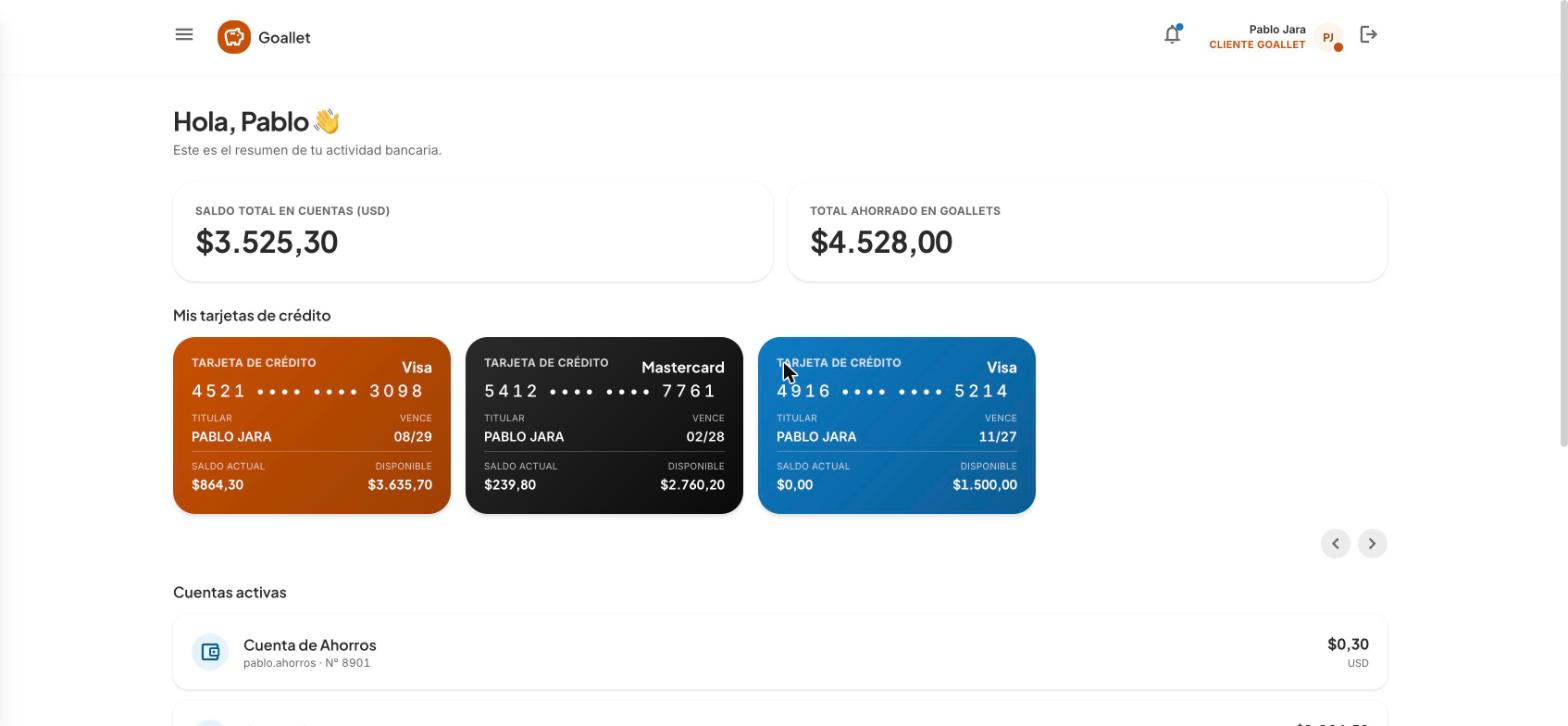
\includegraphics[width=0.9\linewidth]{../evidencias/fase-4-despliegue-frontend/02-dashboard.jpg}
\caption{Dashboard con los saldos de las cuentas obtenidos del Core}\label{fig:e2e-dashboard}
\end{figure}

\begin{figure}[H]
\centering
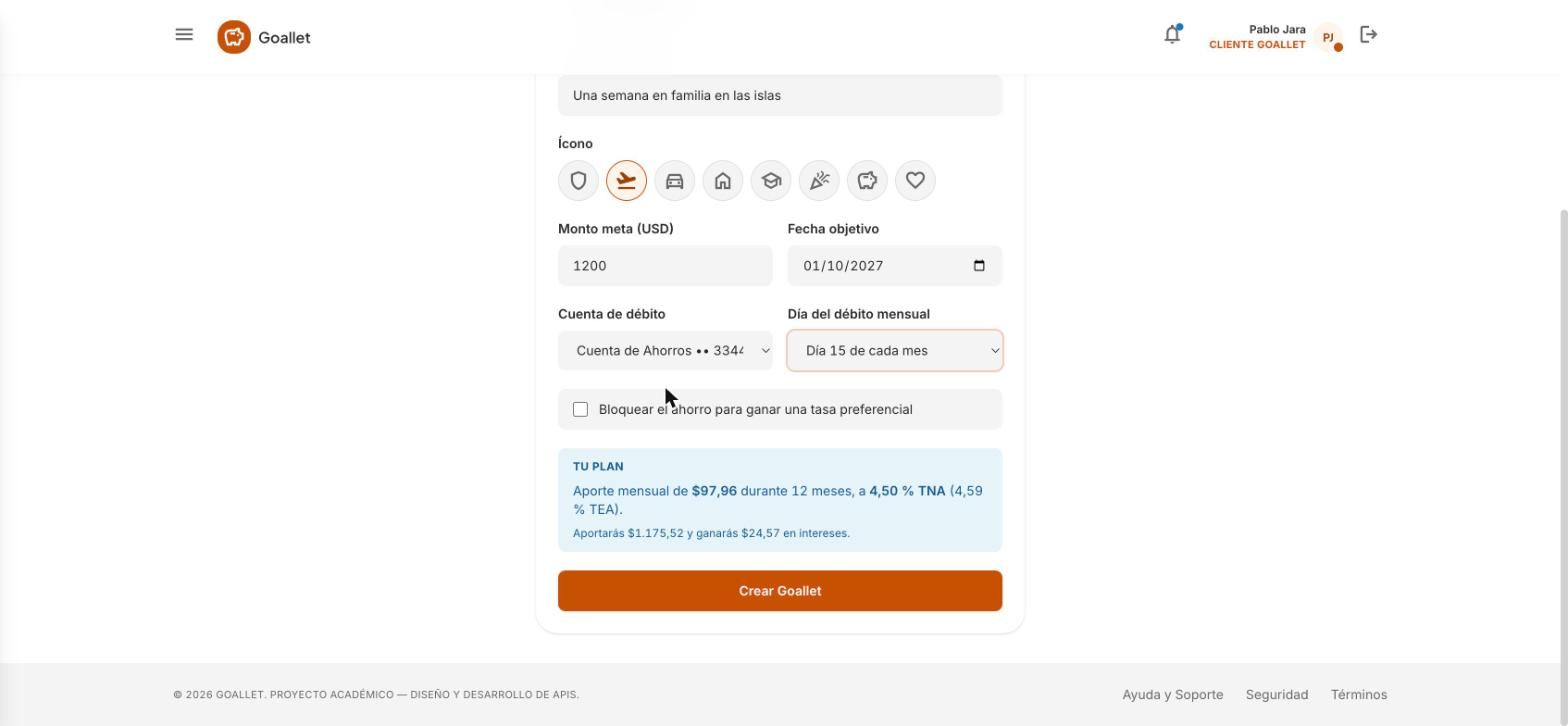
\includegraphics[width=0.9\linewidth]{../evidencias/fase-4-despliegue-frontend/04-nuevo-plan-simulacion.jpg}
\caption{Nuevo plan con la simulación calculada por la API}\label{fig:e2e-simulacion}
\end{figure}

\begin{figure}[H]
\centering
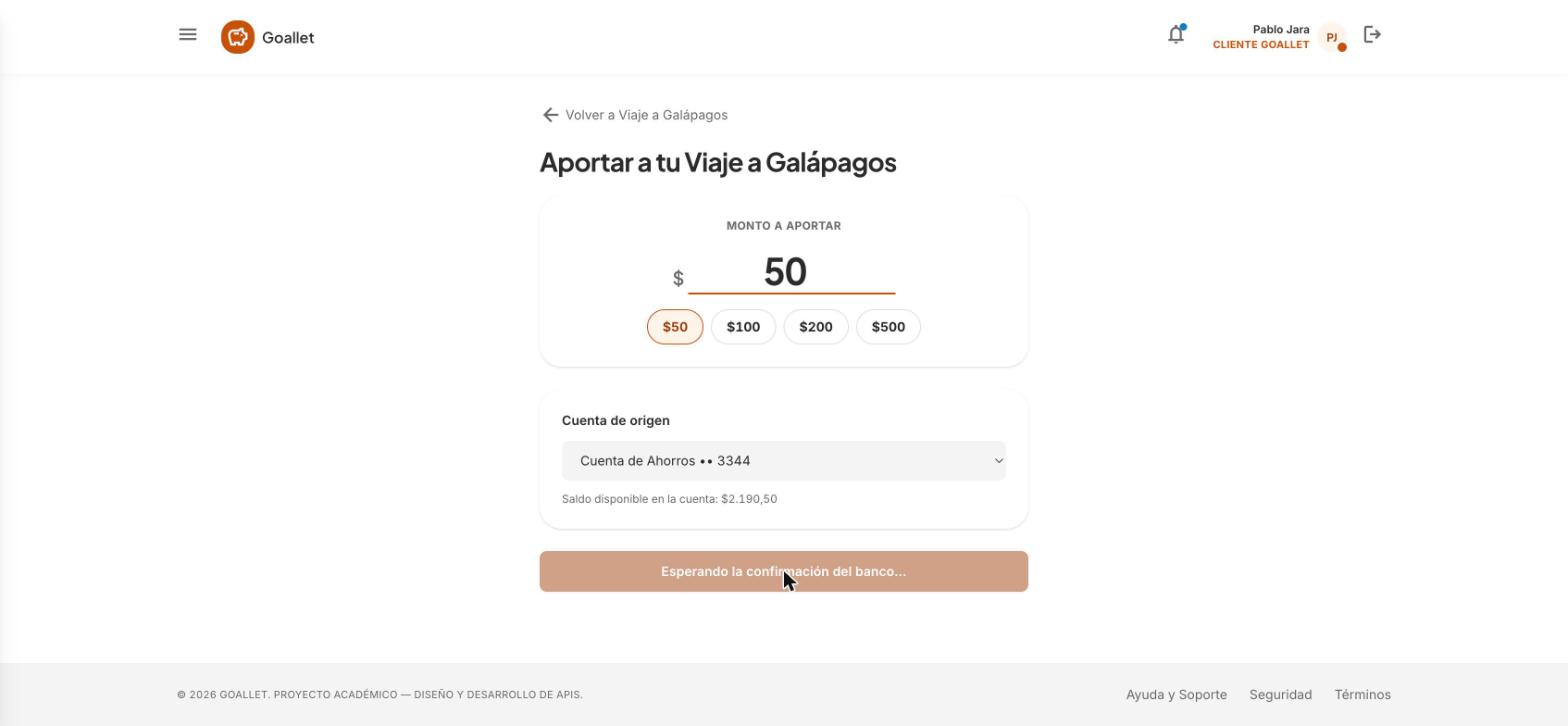
\includegraphics[width=0.9\linewidth]{../evidencias/fase-4-despliegue-frontend/07-aporte-esperando-core.jpg}
\caption{Aporte aceptado (202) a la espera de la confirmación del Core}\label{fig:e2e-pendiente}
\end{figure}

\begin{figure}[H]
\centering
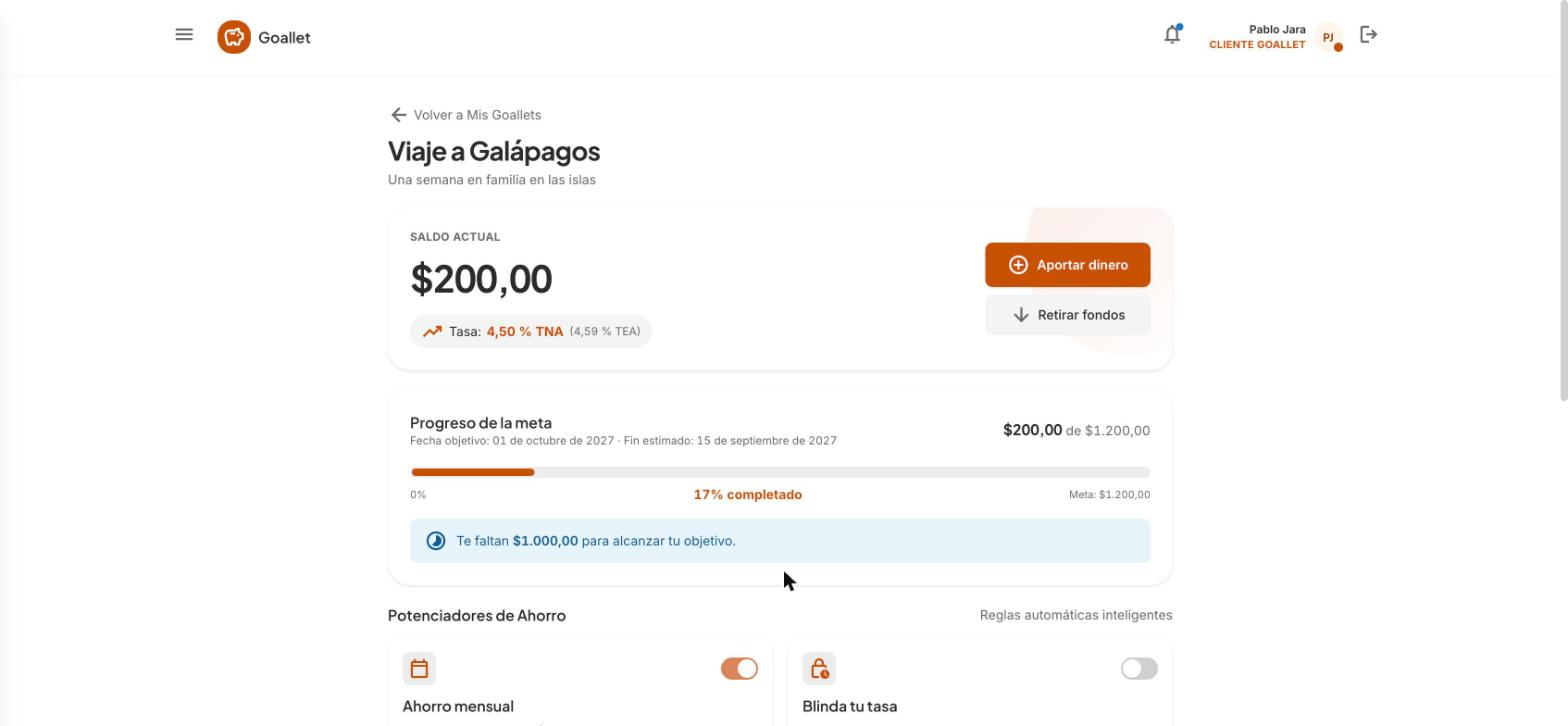
\includegraphics[width=0.9\linewidth]{../evidencias/fase-4-despliegue-frontend/08-aporte-confirmado.jpg}
\caption{Saldo actualizado después de la confirmación del aporte}\label{fig:e2e-aporte}
\end{figure}

\begin{figure}[H]
\centering
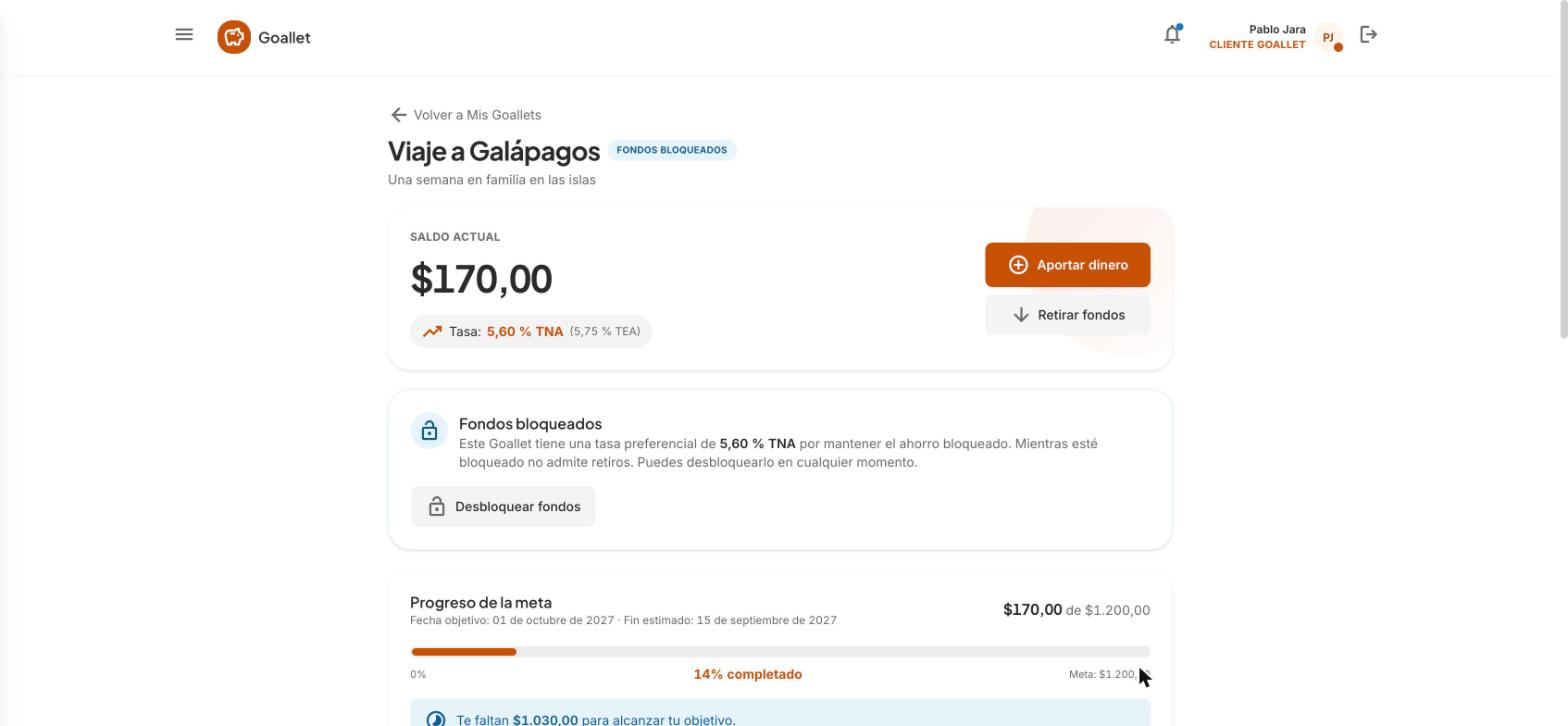
\includegraphics[width=0.9\linewidth]{../evidencias/fase-4-despliegue-frontend/11-plan-bloqueado.jpg}
\caption{Plan bloqueado con la tasa preferencial}\label{fig:e2e-bloqueo}
\end{figure}

\begin{figure}[H]
\centering
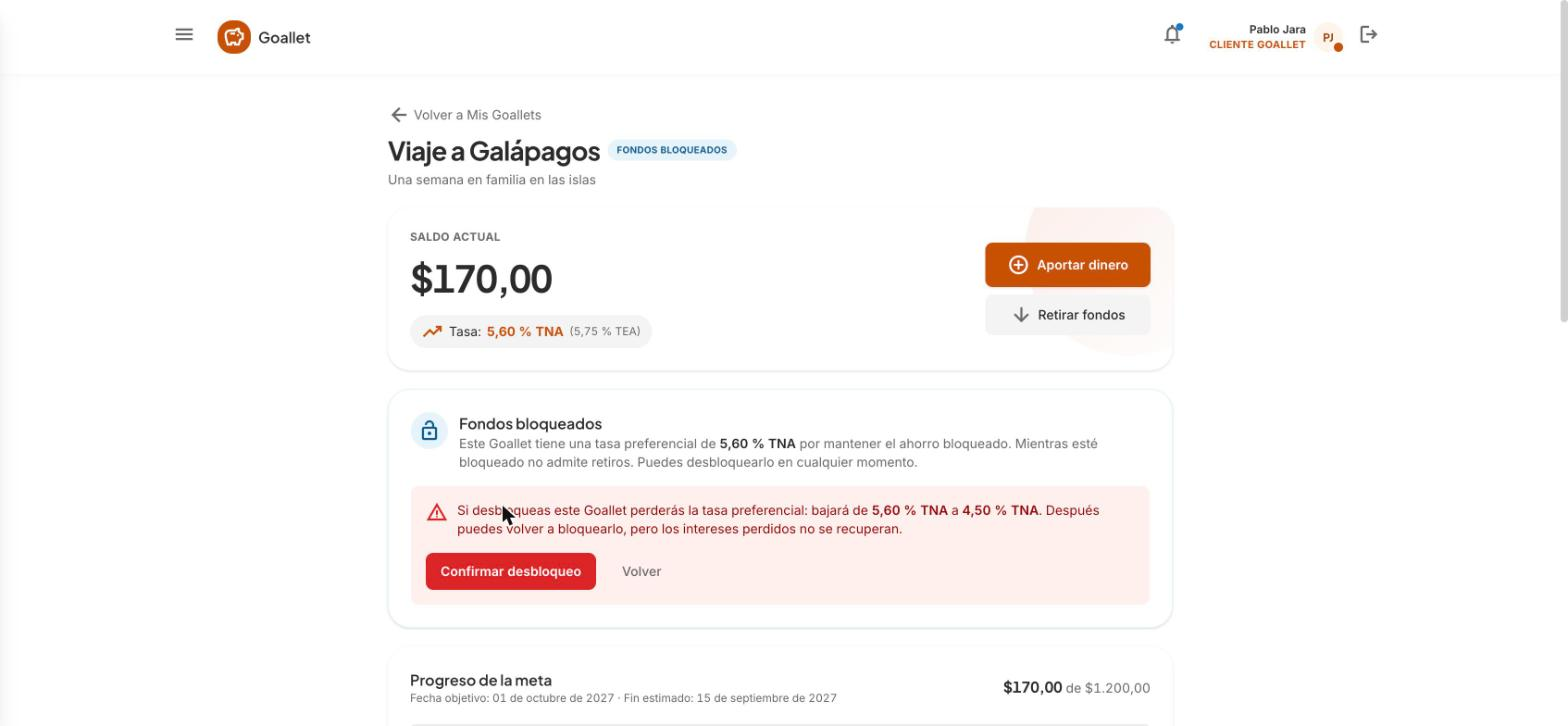
\includegraphics[width=0.9\linewidth]{../evidencias/fase-4-despliegue-frontend/12-desbloqueo-confirmacion.jpg}
\caption{Advertencia antes de desbloquear el plan}\label{fig:e2e-desbloqueo}
\end{figure}

\begin{figure}[H]
\centering
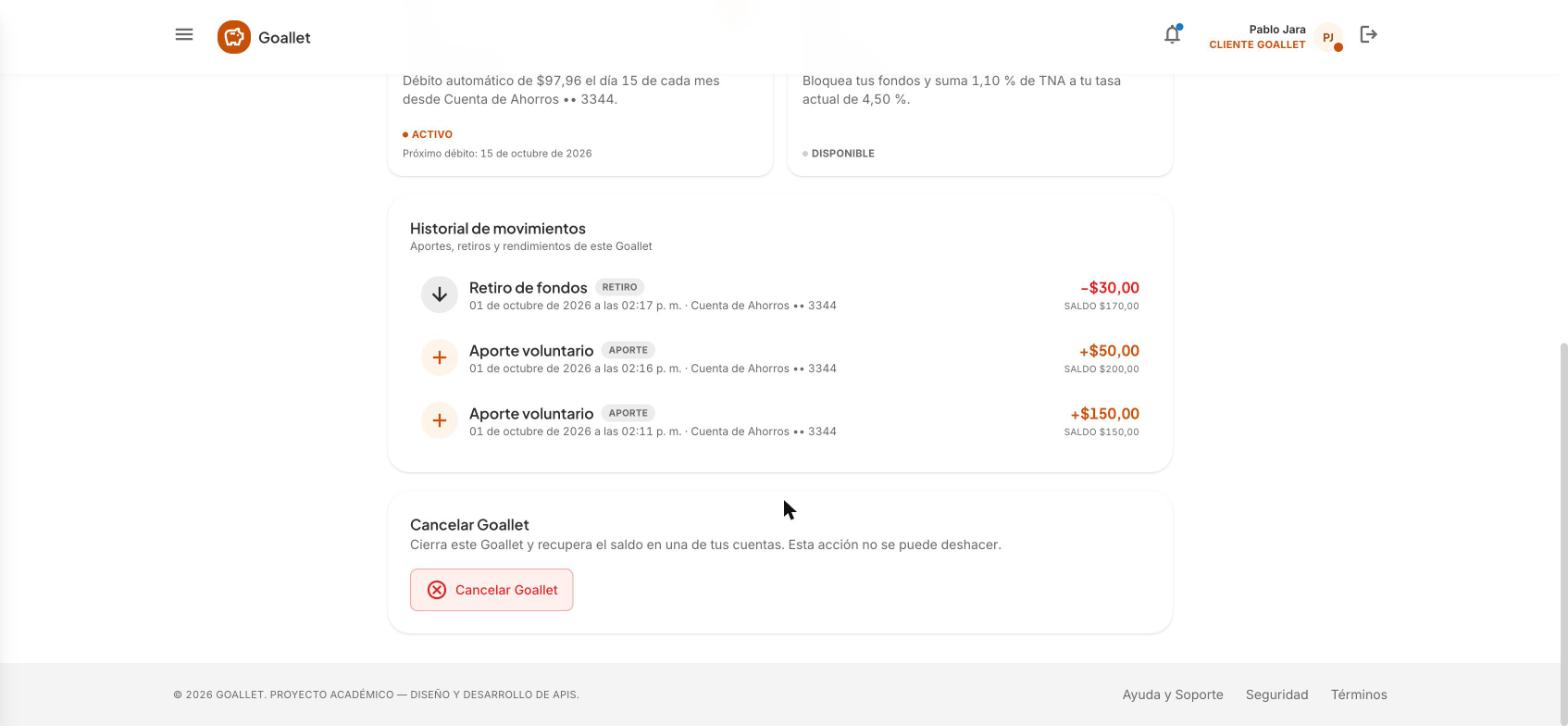
\includegraphics[width=0.9\linewidth]{../evidencias/fase-4-despliegue-frontend/14-historial-movimientos.jpg}
\caption{Historial de movimientos paginado por cursor}\label{fig:e2e-historial}
\end{figure}

\begin{figure}[H]
\centering
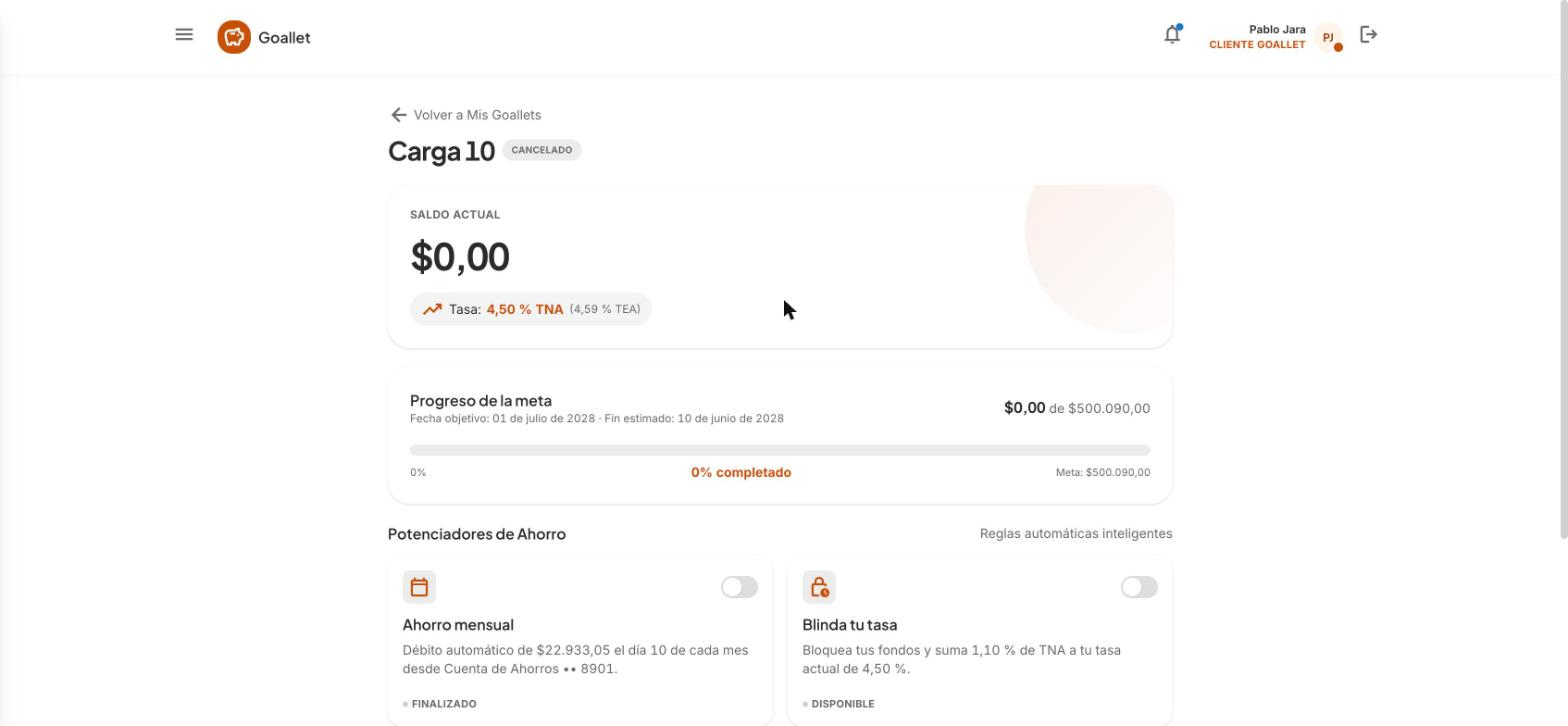
\includegraphics[width=0.9\linewidth]{../evidencias/fase-4-despliegue-frontend/17-plan-cancelado.jpg}
\caption{Plan cancelado}\label{fig:e2e-cancelado}
\end{figure}

Las 17 capturas del recorrido completo están en \texttt{docs/evidencias/fase-4-despliegue-frontend/}.
